% This is samplepaper.tex, a sample chapter demonstrating the
% LLNCS macro package for Springer Computer Science proceedings;
% Version 2.21 of 2022/01/12
%
\documentclass[runningheads]{llncs}
%
\usepackage[T1]{fontenc}
% T1 fonts will be used to generate the final print and online PDFs,
% so please use T1 fonts in your manuscript whenever possible.
% Other font encondings may result in incorrect characters.
%
\usepackage{graphicx}
% Used for displaying a sample figure. If possible, figure files should
% be included in EPS format.
%
% If you use the hyperref package, please uncomment the following two lines
% to display URLs in blue roman font according to Springer's eBook style:
%\usepackage{color}
%\renewcommand\UrlFont{\color{blue}\rmfamily}
%\urlstyle{rm}
%
\begin{document}
%
\title{Visualization of Lattice-Based Cryptanalysis Algorithms}
%
%\titlerunning{Abbreviated paper title}
% If the paper title is too long for the running head, you can set
% an abbreviated paper title here
%
\author{Muhammad Imam Chaidar Mujaddid Al-Ghiffari\inst{1}\orcidID{0000-1111-2222-3333} \and
Second Author\inst{2,3}\orcidID{1111-2222-3333-4444}}
%
\authorrunning{F. Author et al.}
% First names are abbreviated in the running head.
% If there are more than two authors, 'et al.' is used.
%
\institute{Fakultas Ilmu Komputer Universitas Indonesia, Jl. Prof. DR. Sudjono D. Pusponegoro, Pondok Cina, Kecamatan Beji, Kota Depok, Jawa Barat 16425 
\email{https://cs.ui.ac.id/}}
%
\maketitle              % typeset the header of the contribution
%
\begin{abstract}
The abstract should briefly summarize the contents of the paper in
150--250 words.

\keywords{Cryptography  \and Cryptanalisis \and Post-Quantum \and Lattice \and LLL \and BKZ.}
\end{abstract}
%
%
%
\section{Background}

Cryptanalysis is the technique of analysing and breaking a ciphertext to obtain the plaintext (A. Al-Sabaawi, 2020). The history and the development of cryptanalysis itself can't be separated from the history and development of cryptography. As the cryptography techniques evolve, the cryptanalysis techniques also evolve in order to break the cryptography techniques. 

One of the earliest known recorded cryptanalysis technique is the frequency analysis technique, which was used by Arab mathematician Al-Kindi in the 9th century to break monoalphabetic substitution ciphers. This technique relies on the fact that in any given language, certain letters and combinations of letters occur with varying frequencies. By analysing the frequency of letters in the ciphertext, a cryptanalyst can make deduce the likely substitutions used in the cipher.

The frequency analysis technique was arguably the most common and efficient cryptanalysis technique used for breaking classic ciphers. However, as the cipher techniques became more complex, this cryptanalysis technique became less effective. Overall, during and after World War II, mathematics became more and more crucial in both cryptography and cryptanalysis. And the modern cryptanalysis techniques are mostly based on complex mathematical concepts and algorithms, like number theory, algebra, and probability theory.

Since the most common form of modern cryptography is key-based cryptography (symmetric and asymmetric), with the onset of the development of quantum computing and subsequently quantum cryptanalysis, many commonly used modern cryptographic algorithms are threatened by quantum cryptanalysis. For example, Shor's algorithm - a quantum algorithm to finding prime factors of an integer, can efficiently factor large integers and compute discrete logarithms. Which endangers the security of commonly used asymmetric cryptographic algorithms like RSA and ECC. Not only asymmetric cryptographic algorithms are threatened by this, Grover's algorithm - also known as Quantum Search Algorithm, can search unsorted databases quadratically faster than classical algorithms, which threatens the security of symmetric-key cryptosystems by effectively halving their key lengths. 

Which is why cryptographers around the world already started to develop cryptographic algorithms that can resist quantum cryptanalysis. These newer and stronger cryptographic algorithms are called post-quantum cryptography (PQC). Examples of PQC algorithms include Kyber and Dilithium, which are based on the hardness of lattice problems. In fact, lattice-based cryptographic algorithms dominate the PQC. The lattice-based PQC algorithms are indeed able to resist quantum computer-based cryptanalysis. For example, the quantum cryptanalysis technique of Shor's Algorithm can't break it efficiently.

However, just like how the historical pattern of cryptanalysis and cryptography goes in our history, as cryptographers developed lattice-based cryptographic algorithms, the cryptanalysis experts also developed lattice-based cryptanalysis techniques in order to break the lattice-based cryptographic algorithms. The most common lattice-based cryptanalysis technique is the LLL algorithm, which is a polynomial-time algorithm for finding a short and nearly orthogonal basis for a lattice. This algorithm can be used to solve the shortest vector problem (SVP) and the closest vector problem (CVP), which are both important issues in lattice-based cryptography. Apparently, for now, the most promising lattice-based cryptanalysis technique is the BKZ algorithm, which is basically the upscaled version of the LLL algorithm. Compared to LLL, BKZ can find even shorter vectors in a lattice.

The problem with these lattice-based cryptanalysis techniques is that in general, they are very complex and hard to understand, especially for people who are new to the field of cryptography and cryptanalysis. This is where the visualization of these algorithms can be very helpful. However, most visualizations of these algorithms don't visualize the underlying mathematical concepts in an intuitive way. By visualizing these algorithms in an intuitive way, we can make them easier to understand and more accessible to a wider audience. 

\section{Related Works}

\subsection{lll-attack-runner}

\subsection{fpylll}

\subsection{x}

\section{Architecture}

\subsection{Backend}
We will use Zachary Robert Bennett's lll-attack-runner, which is an interactive, largely Javascript-based lattice-based cryptanalysis solveR, as the backend for our visualization of the LLL and BKZ algorithms.

\subsection{Frontend}
For the frontend part, we wil use Next.js, which is a React-based framework for building web applications. The usage of Next.js is intended to create a user-friendly interface for our visualization of the LLL and BKZ algorithms. The frontend will allow users to input their own lattice-based cryptanalysis problems and visualize the steps of the LLL and BKZ algorithms in an intuitive way.

\subsection{A Subsection Sample}
Please note that the first paragraph of a section or subsection is
not indented. The first paragraph that follows a table, figure,
equation etc. does not need an indent, either.

Subsequent paragraphs, however, are indented.

\subsubsection{Sample Heading (Third Level)} Only two levels of
headings should be numbered. Lower level headings remain unnumbered;
they are formatted as run-in headings.

\paragraph{Sample Heading (Fourth Level)}
The contribution should contain no more than four levels of
headings. Table~\ref{tab1} gives a summary of all heading levels.

\begin{table}
\caption{Table captions should be placed above the
tables.}\label{tab1}
\begin{tabular}{|l|l|l|}
\hline
Heading level &  Example & Font size and style\\
\hline
Title (centered) &  {\Large\bfseries Lecture Notes} & 14 point, bold\\
1st-level heading &  {\large\bfseries 1 Introduction} & 12 point, bold\\
2nd-level heading & {\bfseries 2.1 Printing Area} & 10 point, bold\\
3rd-level heading & {\bfseries Run-in Heading in Bold.} Text follows & 10 point, bold\\
4th-level heading & {\itshape Lowest Level Heading.} Text follows & 10 point, italic\\
\hline
\end{tabular}
\end{table}


\noindent Displayed equations are centered and set on a separate
line.
\begin{equation}
x + y = z
\end{equation}
Please try to avoid rasterized images for line-art diagrams and
schemas. Whenever possible, use vector graphics instead (see
Fig.~\ref{fig1}).

\begin{figure}
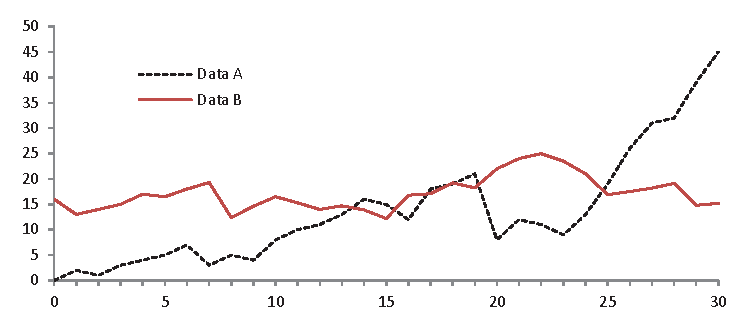
\includegraphics[width=\textwidth]{fig1.eps}
\caption{A figure caption is always placed below the illustration.
Please note that short captions are centered, while long ones are
justified by the macro package automatically.} \label{fig1}
\end{figure}

\begin{theorem}
This is a sample theorem. The run-in heading is set in bold, while
the following text appears in italics. Definitions, lemmas,
propositions, and corollaries are styled the same way.
\end{theorem}
%
% the environments 'definition', 'lemma', 'proposition', 'corollary',
% 'remark', and 'example' are defined in the LLNCS documentclass as well.
%
\begin{proof}
Proofs, examples, and remarks have the initial word in italics,
while the following text appears in normal font.
\end{proof}
For citations of references, we prefer the use of square brackets
and consecutive numbers. Citations using labels or the author/year
convention are also acceptable. The following bibliography provides
a sample reference list with entries for journal
articles~\cite{ref_article1}, an LNCS chapter~\cite{ref_lncs1}, a
book~\cite{ref_book1}, proceedings without editors~\cite{ref_proc1},
and a homepage~\cite{ref_url1}. Multiple citations are grouped
\cite{ref_article1,ref_lncs1,ref_book1},
\cite{ref_article1,ref_book1,ref_proc1,ref_url1}.

\begin{credits}
\subsubsection{\ackname} A bold run-in heading in small font size at the end of the paper is
used for general acknowledgments, for example: This study was funded
by X (grant number Y).

\subsubsection{\discintname}
It is now necessary to declare any competing interests or to specifically
state that the authors have no competing interests. Please place the
statement with a bold run-in heading in small font size beneath the
(optional) acknowledgments\footnote{If EquinOCS, our proceedings submission
system, is used, then the disclaimer can be provided directly in the system.},
for example: The authors have no competing interests to declare that are
relevant to the content of this article. Or: Author A has received research
grants from Company W. Author B has received a speaker honorarium from
Company X and owns stock in Company Y. Author C is a member of committee Z.
\end{credits}
%
% ---- Bibliography ----
%
% BibTeX users should specify bibliography style 'splncs04'.
% References will then be sorted and formatted in the correct style.
%
% \bibliographystyle{splncs04}
% \bibliography{mybibliography}
%
\begin{thebibliography}{8}
\bibitem{ref_article1}
Author, F.: Article title. Journal \textbf{2}(5), 99--110 (2016)

\bibitem{ref_lncs1}
Author, F., Author, S.: Title of a proceedings paper. In: Editor,
F., Editor, S. (eds.) CONFERENCE 2016, LNCS, vol. 9999, pp. 1--13.
Springer, Heidelberg (2016). \doi{10.10007/1234567890}

\bibitem{ref_book1}
Author, F., Author, S., Author, T.: Book title. 2nd edn. Publisher,
Location (1999)

\bibitem{ref_proc1}
Author, A.-B.: Contribution title. In: 9th International Proceedings
on Proceedings, pp. 1--2. Publisher, Location (2010)

\bibitem{ref_url1}
LNCS Homepage, \url{http://www.springer.com/lncs}, last accessed 2023/10/25
\end{thebibliography}
\end{document}
